\ifdefined\PRESENTATION\else\PassOptionsToClass{handout}{beamer}\fi\documentclass[aspectratio=169, lualatex]{beamer}
\makeatletter\def\input@path{{theme/}}\makeatother\usetheme{cipher}

\title{Applied Cryptography - 2.2: The Story of RC4}
\author{Nadim Kobeissi}
\subject{The complete life cycle of a cipher: RC4's design in 1987, its leak in 1994, its rise to dominance in WEP and TLS, the twenty years of cryptanalysis that dismantled it, and its formal prohibition in 2015.}
\keywords{RC4, stream cipher, cryptanalysis, WEP, TLS, FMS attack, statistical biases, ABSAB bias, broadcast attack, RC4 NOMORE, nonce misuse, cryptographic agility}
\institute{Symbolic Software}
\instituteimage{images/symbolicsoft-white.png}
\date{\today}
\coversubtitle{Summer 2026}
\coverpartname{Part 2: Real-World Cryptography}
\covertopicname{2.2: The Story of RC4}
\coverwebsite{https://appliedcryptography.page}

\begin{document}
\begin{frame}[plain]
	\titlepage
\end{frame}

\section{A Cipher Worth Studying}

\begin{frame}{Why spend a lecture on a dead cipher?}
	\begin{itemize}[<+->]
		\item RC4 is the best-documented \textbf{complete life cycle} we have in cryptography: we get to watch a cipher be born, conquer the internet, and die.
		\item Almost nothing else offers this. Most broken ciphers die young and obscure; most surviving ciphers have not finished their story.
		\item \textbf{What we are actually here to learn:}
		      \begin{itemize}
			      \item How a tiny statistical flaw becomes a total break, given enough traffic.
			      \item How a \emph{primitive} can be sound while every \emph{protocol} using it fails.
			      \item How long it takes to remove a broken algorithm from the internet, and why.
		      \end{itemize}
		\item RC4 itself is dead. Every one of its failure modes is alive.
	\end{itemize}
\end{frame}

\begin{frame}{The arc of RC4}
	\begin{itemize}[<+->]
		\item \textbf{1987 --- Birth.} Ron Rivest designs RC4 as a trade secret at RSA Security.
		\item \textbf{1994 --- Escape.} The algorithm is leaked anonymously to the Cypherpunks mailing list.
		\item \textbf{1990s--2000s --- Empire.} The most widely deployed stream cipher in history: WEP, SSL/TLS, SSH-1, Office, PDF.
		\item \textbf{1995--2001 --- Hairline cracks.} Academics find statistical oddities. Nobody panics.
		\item \textbf{2001 --- WEP falls.} Fluhrer--Mantin--Shamir turn an oddity into total Wi-Fi key recovery.
		\item \textbf{2013--2015 --- TLS falls.} Bias attacks recover cookies and passwords from HTTPS.
		\item \textbf{2015 --- Prohibition.} RFC 7465 bans RC4 in TLS; browsers finish the job by 2016.
	\end{itemize}
	\onslide<+->{\centering\textbf{Twenty-eight years from design to formal ban.}}
\end{frame}

\begin{frame}{Where RC4 came from}
	\begin{columns}[c]
		\begin{column}{0.56\textwidth}
			\begin{itemize}[<+->]
				\item \textbf{1987:} Designed by Ron Rivest at RSA Security. ``RC'' for ``Rivest Cipher'' (or ``Ron's Code'').
				      \begin{itemize}
					      \item Kept as a \textbf{trade secret}, never published, licensed only under NDA.
				      \end{itemize}
				\item \textbf{September 1994:} the algorithm is posted anonymously to the Cypherpunks mailing list.
				      \begin{itemize}
					      \item Verified against licensed implementations within days.
					      \item RSA never confirmed it, so the public version was politely called \textbf{``Alleged RC4''} or \textbf{ARCFOUR} --- a name still in OpenSSH and GnuTLS today.
				      \end{itemize}
			\end{itemize}
		\end{column}
		\begin{column}{0.44\textwidth}
			\onslide<+->{
				\definitionbox{Security by obscurity}{
					Seven years of secrecy bought RSA nothing. The design leaked in a single message, and the weaknesses were found \emph{after} publication, by the open research community RSA had excluded.
					\vspace{0.5em}
					\\
					Note the irony: the leak is what made RC4 ubiquitous. Free availability, not licensing, built the empire.
				}
			}
		\end{column}
	\end{columns}
\end{frame}

\begin{frame}{Why everyone chose RC4}
	\begin{columns}[c]
		\begin{column}{0.54\textwidth}
			\begin{itemize}[<+->]
				\item \textbf{Fast in software.} Around an order of magnitude quicker than DES.
				\item \textbf{Tiny.} 256 bytes of state and two indices. It fits on a microcontroller.
				\item \textbf{Trivial to implement.} Roughly ten lines of code. Compare with a correct AES.
				\item \textbf{No blocks, no padding.} $n$ bytes in, $n$ bytes out.
				\item \textbf{Export-friendly.} At 40 bits it cleared US export controls, so one codebase shipped worldwide.
			\end{itemize}
		\end{column}
		\begin{column}{0.46\textwidth}
			\onslide<+->{
				\textbf{Where it ended up:}
				\begin{itemize}
					\item \textbf{WEP} (1997): Wi-Fi, RC4 exclusively.
					\item \textbf{SSL 3.0 / TLS 1.0}: preferred suite for years.
					\item \textbf{SSH-1} (1995): \texttt{arcfour}.
					\item \textbf{Office} and \textbf{PDF}: document encryption.
					\item \textbf{Kerberos}: \texttt{RC4-HMAC}, still limping along.
				\end{itemize}
			}
			\onslide<+->{\centering At its peak, RC4 protected roughly \textbf{half of all TLS traffic}.}
		\end{column}
	\end{columns}
\end{frame}

\section{How RC4 Works}

\begin{frame}{Idea: find a way to expand the key}{Reminder}
	\begin{itemize}
		\item Given a key $k_s$ of size $\left|k_s\right| < \left|m\right|$, find a way to obtain a key $k_e$ where $\left|k_e\right| \geq \left|m\right|$.
		\item In the real world, we have two kinds of symmetric encryption schemes:
		      \begin{itemize}
			      \item \textbf{Block ciphers}: AES, 3DES, etc.
			      \item \textbf{Stream ciphers}: ChaCha20, RC4, etc.
		      \end{itemize}
		\item This is exactly what stream ciphers do!
		      \begin{itemize}
			      \item Start with a small key $k_s$ of a fixed size $\left|k_s\right| = \lambda$,
			      \item Magically expand it to $k_e$ where $\left|k_e\right| \geq \left|m\right|$,
			      \item $\func{enc}{k_e, M} = k_e \oplus M$
		      \end{itemize}
		\item \textbf{RC4 is one answer to ``how do we do the magic?''}
	\end{itemize}
\end{frame}

\begin{frame}{RC4 is two algorithms}
	\begin{columns}[t]
		\begin{column}{0.5\textwidth}
			\begin{center}
				\sssubroutine{RC4.KSA}{k}{
					for $i \coloneq 0$ to $255$: \\
					\quad $S[i] \coloneq i$ \\
					$j \coloneq 0$ \\
					for $i \coloneq 0$ to $255$: \\
					\quad $j \coloneq (j + S[i] + k[i \bmod |k|]) \bmod 256$ \\
					\quad swap $S[i]$, $S[j]$ \\
					return $S$
				}{0.74}
			\end{center}
			\begin{itemize}
				\item \textbf{Key Scheduling:} stir the key into a permutation of $0..255$.
			\end{itemize}
		\end{column}
		\begin{column}{0.5\textwidth}
			\begin{center}
				\sssubroutine{RC4.PRGA}{S}{
					$i \coloneq 0$, \quad $j \coloneq 0$ \\
					loop: \\
					\quad $i \coloneq (i + 1) \bmod 256$ \\
					\quad $j \coloneq (j + S[i]) \bmod 256$ \\
					\quad swap $S[i]$, $S[j]$ \\
					\quad yield $S[(S[i] + S[j]) \bmod 256]$
				}{0.74}
			\end{center}
			\begin{itemize}
				\item \textbf{Generation:} one keystream byte per iteration.
				\item $\func{Enc}{k, M} = M \oplus \texttt{RC4}(k)$, and decryption is the same function.
			\end{itemize}
		\end{column}
	\end{columns}
\end{frame}

\begin{frame}{The state is always a permutation}
	\begin{columns}[c]
		\begin{column}{0.5\textwidth}
			\begin{itemize}[<+->]
				\item $S$ starts as the identity permutation and \textbf{every operation is a swap}, so $S$ stays a permutation forever: no value is lost or duplicated.
				\item The KSA's whole job is to make it look uniformly drawn from all $256!$ of them. \textbf{Every attack in this lecture says the same thing:} it does not quite manage it.
				\item \textbf{Careful:} $S$ is a permutation, but RC4 is \emph{not} a PRP. It is a PRG --- seed in, keystream out.
			\end{itemize}
		\end{column}
		\begin{column}{0.5\textwidth}
			\begin{center}
				\begin{tikzpicture}[scale=0.33]
					\definecolor{domaingreen}{RGB}{102, 170, 68}
					\definecolor{circlecolor}{RGB}{235, 137, 85}
					\definecolor{purplearrow}{RGB}{160, 78, 160}

					\draw[dashed, thick, domaingreen, fill=domaingreen] (0,0) rectangle (8,8);
					\node[font=\small] at (4,9.2) {Indices $0..255$};

					\draw[thick, domaingreen, fill=domaingreen] (12,0) rectangle (20,8);
					\node[font=\small] at (16,9.2) {Values $0..255$};

					\filldraw[circlecolor] (2,7) circle (0.3);
					\draw[-{Stealth[length=3mm, width=2mm]}, thick, purplearrow] (2,7) -- (14.2,7.4);
					\filldraw[circlecolor] (14.2,7.4) circle (0.3);

					\filldraw[circlecolor] (3,6) circle (0.3);
					\draw[-{Stealth[length=3mm, width=2mm]}, thick, purplearrow] (3,6) -- (18.6,5.3);
					\filldraw[circlecolor] (18.6,5.3) circle (0.3);
					\pause

					\filldraw[circlecolor] (2,5) circle (0.3);
					\draw[-{Stealth[length=3mm, width=2mm]}, thick, purplearrow] (2,5) -- (13.8,4.2);
					\filldraw[circlecolor] (13.8,4.2) circle (0.3);

					\filldraw[circlecolor] (4,3.5) circle (0.3);
					\draw[-{Stealth[length=3mm, width=2mm]}, thick, purplearrow] (4,3.5) -- (17.4,2.2);
					\filldraw[circlecolor] (17.4,2.2) circle (0.3);
					\pause

					\filldraw[circlecolor] (2,2) circle (0.3);
					\draw[-{Stealth[length=3mm, width=2mm]}, thick, purplearrow] (2,2) -- (16.1,6.7);
					\filldraw[circlecolor] (16.1,6.7) circle (0.3);

					\filldraw[circlecolor] (3,1) circle (0.3);
					\draw[-{Stealth[length=3mm, width=2mm]}, thick, purplearrow] (3,1) -- (19.0,1.4);
					\filldraw[circlecolor] (19.0,1.4) circle (0.3);
				\end{tikzpicture}
				\\[0.6em]
				\small Bijective: no collisions, nothing unmapped.
			\end{center}
		\end{column}
	\end{columns}
\end{frame}

\begin{frame}{The flaw that explains this entire lecture}
	\begin{columns}[c]
		\begin{column}{0.4\textwidth}
			\begin{center}
				\large
				$\texttt{ChaCha20}(\underbrace{K}_{\text{secret}}, \underbrace{N}_{\text{per message}}, \text{ctr})$
				\\[1.2em]
				$\texttt{RC4}(\underbrace{k}_{\text{secret}})$
			\end{center}
			\vspace{0.5em}
			\onslide<2->{
				\alertbox{RC4 has no nonce}{
					There is nowhere to put a per-message value. The keystream is a function of the key and \emph{nothing else}.
				}
			}
		\end{column}
		\begin{column}{0.6\textwidth}
			\begin{itemize}[<3->]
				\item One key must never produce the same keystream twice. Modern ciphers use a \textbf{nonce}: same $K$, different $N$, unrelated keystream.
				\item RC4 offers no such input, so every protocol had to \textbf{invent one} by manufacturing a fresh $k$ per message.
				\item \textbf{WEP's answer:} $k \coloneq IV \,\|\, K$. Cheap, and catastrophic.
				\item \textbf{TLS's answer:} a fresh $k$ per connection, from the handshake. Sound! But then the \emph{same} plaintext is encrypted under many keys.
			\end{itemize}
			\onslide<7->{\centering\textbf{One missing input, two different catastrophes.}}
		\end{column}
	\end{columns}
\end{frame}

\section{The Cracks Appear}

\begin{frame}{Early warnings (1995--2001)}
	\begin{itemize}[<+->]
		\item \textbf{1995 --- Roos.} The first bytes of $S$ after the KSA are correlated with the first bytes of the key, and a class of \textbf{weak keys} leaves structure that survives into the keystream.
		      \begin{itemize}
			      \item Published to \texttt{sci.crypt}, not to a conference. Treated as a curiosity.
		      \end{itemize}
		\item \textbf{1996 --- Jenkins' ``Glimpse'' theorem.} Each keystream byte leaks the internal state: $\Pr[S[j] = i - Z] \approx 2/256$, twice what it should be.
		\item \textbf{1997 --- Goli\'{c} (Eurocrypt).} A linear statistical weakness in the output, giving a distinguisher from random.
		\item \textbf{2001 --- Mantin \& Shamir (FSE).} The cleanest result of the era, and the one that should have ended RC4 on the spot.
	\end{itemize}
	\onslide<+->{\centering\textit{Every one of these was published, peer-reviewed, and deployed straight past.}}
\end{frame}

\begin{frame}{Mantin \& Shamir (2001): the second byte betrays you}
	\begin{columns}[c]
		\begin{column}{0.52\textwidth}
			\begin{itemize}[<+->]
				\item \textbf{The theorem:} if after the KSA we have $S[2] = 0$ and $S[1] \neq 2$, then the second keystream byte is \textbf{always} $Z_2 = 0$.
				\item That precondition holds for about $1$ key in $256$. When it fails, $Z_2 = 0$ still happens by chance $1$ time in $256$.
				\item So $\Pr[Z_2 = 0] \approx \frac{2}{256}$: \textbf{double} the correct probability, for a perfectly random key.
			\end{itemize}
		\end{column}
		\begin{column}{0.48\textwidth}
			\onslide<+->{
				\definitionbox{Why this is devastating}{
					Take one plaintext byte encrypted under many independent keys --- say, byte 2 of a cookie sent on every request.
					\vspace{0.5em}
					\\
					The most common ciphertext byte at position 2 is $M_2 \oplus 0 = M_2$.
					\vspace{0.5em}
					\\
					\textbf{You do not need the key. You only need to count.}
				}
			}
			\onslide<+->{\centering This is the \textbf{broadcast attack}. It sat in the literature for twelve years before anyone aimed it at TLS.}
		\end{column}
	\end{columns}
\end{frame}

\begin{frame}{One-time secrecy of an SKE}{Reminder}
	\begin{columns}[c]
		\begin{column}{0.5\textwidth}
			\definitionbox{One-time Secrecy for SKE}{
				An SKE scheme $\Sigma$ has one-time secrecy if the following libraries are interchangeable:
				\vspace{0.5mm}
				\begin{center}
					\sslinked{
						\sslibrary{\Sigma}{ots-real}{
							\sslibrarysubroutine{ots.enc}{M}{
								$K \twoheadleftarrow \Sigma.\mathcal{K}$ \\
								$C \coloneq \Sigma.\textsf{Enc}(K, M)$ \\
								return $C$
							}{1}
						}{0.8}
					}{\interchangeable{}}{
						\sslibrary{\Sigma}{ots-rand}{
							\sslibrarysubroutine{ots.enc}{M}{
								$C \twoheadleftarrow \Sigma.\mathcal{C}$ \\
								return $C$
							}{1}
						}{0.8}
					}
				\end{center}
			}
		\end{column}
		\begin{column}{0.5\textwidth}
			An encryption scheme has one-time secrecy if its ciphertexts are uniformly distributed when keys are sampled uniformly, kept secret, and used for only one encryption, no matter how the plaintexts are chosen.
			\\[1em]
			\textbf{Mantin and Shamir just handed us a distinguisher between these two libraries:} call \textsf{ots.enc} on a fixed $M$ a few million times, and count how often byte 2 of $C$ equals $M_2$.
		\end{column}
	\end{columns}
\end{frame}

\begin{frame}{Attacks mean distinguishability}{RC4 getting less and less ``indistinguishable from random''}
	\begin{columns}[c]
		\begin{column}{0.35\textwidth}
			\sssubroutine{RC4Encrypt}{M}{
				$k \twoheadleftarrow \bits^{\lambda}$ \\
				$K \coloneq \texttt{RC4}(k, |M|)$ \\
				$C \coloneq K \oplus M$ \\
				return $C$
			}{1.2}
		\end{column}
		\begin{column}{0.3\textwidth}
			\begin{center}
				{\huge{$\cancel{\approxeq}$}}
			\end{center}
		\end{column}
		\begin{column}{0.35\textwidth}
			\sssubroutine{Random}{M}{
				$C \twoheadleftarrow \bits^{|M|}$ \\
				return $C$
			}{1.2}
		\end{column}
	\end{columns}
	\begin{itemize}
		\item A ``bias'' is not a soft, qualitative complaint. It is a \textbf{concrete distinguisher}, and therefore a proof that the scheme fails our definition.
		\item The only question left is how many samples that distinguisher needs.
	\end{itemize}
\end{frame}

\begin{frame}{In fact\ldots}
	\begin{center}
		\vspace{-0.3em}
		\begin{tikzpicture}
			\node[fill=white, anchor=center, inner sep=1mm]{
				\includegraphics[height=0.68\textheight, keepaspectratio]{images/rc4-bias.png}
			};
			\node[fit=(current bounding box), inner sep=0.5mm, draw=white, line width=0.5mm] {};
		\end{tikzpicture}
		\\[0.2em]
		{\usebeamerfont{caption} Position across, byte value up, colour showing deviation from uniform. A good stream cipher would be a flat, featureless field. Source: Kenny Paterson.}
	\end{center}
\end{frame}

\section{RC4 in WEP}

\begin{frame}{How WEP encryption works}
	\begin{columns}[c]
		\begin{column}{0.44\textwidth}
			\begin{itemize}
				\item \textbf{A 104-bit key $K$}, shared by every device on the network.
				      \begin{itemize}
					      \item Typed in as hex or ASCII, \emph{not} run through a KDF. Originally 40 bits, for US export controls.
				      \end{itemize}
				\item \textbf{A 24-bit IV}, chosen per packet.
				\item \textbf{Per packet:} form the RC4 key $IV \,\|\, K$, XOR the keystream with the plaintext, and send the IV \textbf{in the clear}.
			\end{itemize}
			\begin{center}
				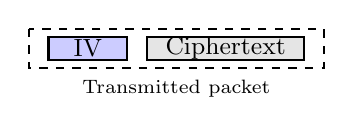
\begin{tikzpicture}[scale=0.5]
					\draw[thick, dashed] (-0.5,-0.5) rectangle (7,-1.5);
					\draw[thick, fill=blue!20] (0,-0.7) rectangle (2,-1.3);
					\node at (1,-1) {\small IV};
					\draw[thick, fill=gray!20] (2.5,-0.7) rectangle (6.5,-1.3);
					\node at (4.5,-1) {\small Ciphertext};
					\node[below] at (3.25,-1.55) {\scriptsize Transmitted packet};
				\end{tikzpicture}
			\end{center}
		\end{column}
		\begin{column}{0.56\textwidth}
			\begin{center}
				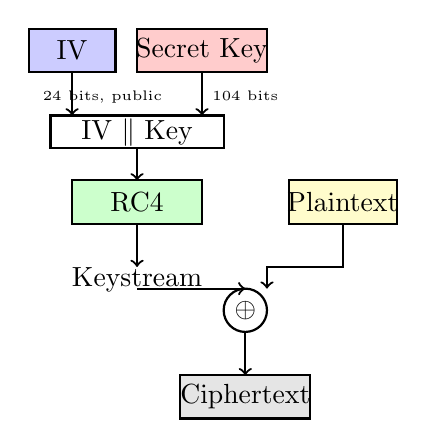
\begin{tikzpicture}[scale=0.55]
					\draw[thick, fill=blue!20] (0,4) rectangle (2,5);
					\node at (1,4.5) {IV};
					\node[below] at (1.7,3.8) {\tiny 24 bits, public};

					\draw[thick, fill=red!20] (2.5,4) rectangle (5.5,5);
					\node at (4,4.5) {Secret Key};
					\node[below] at (5,3.8) {\tiny 104 bits};

					\draw[->, thick] (1,4) -- (1,3);
					\draw[->, thick] (4,4) -- (4,3);
					\draw[thick] (0.5,2.25) rectangle (4.5,3);
					\node at (2.5,2.6) {IV $\|$ Key};

					\draw[->, thick] (2.5,2.25) -- (2.5,1.5);
					\draw[thick, fill=green!20] (1,0.5) rectangle (4,1.5);
					\node at (2.5,1) {RC4};

					\draw[->, thick] (2.5,0.5) -- (2.5,-0.5);
					\node at (2.5,-0.8) {Keystream};

					\draw[thick, fill=yellow!20] (6,0.5) rectangle (8.5,1.5);
					\node at (7.25,1) {Plaintext};

					\draw[->, thick] (2.5,-1) -- (5,-1);
					\draw[->, thick] (7.25,0.5) -- (7.25,-0.5) -- (5.5,-0.5) -- (5.5,-1);
					\draw[thick] (5,-1.5) circle (0.5);
					\node at (5,-1.5) {$\oplus$};

					\draw[->, thick] (5,-2) -- (5,-3);
					\draw[thick, fill=gray!20] (3.5,-3) rectangle (6.5,-4);
					\node at (5,-3.5) {Ciphertext};
				\end{tikzpicture}
			\end{center}
		\end{column}
	\end{columns}
\end{frame}

\begin{frame}{WEP: the perfect storm}
	\begin{itemize}[<+->]
		\item WEP needed a per-packet keystream and RC4 has no nonce, so WEP concatenated: the RC4 key is $(IV_1, IV_2, IV_3, K_1, K_2, \ldots, K_{13})$.
		\item Look at what that hands an attacker, for free:
		      \begin{itemize}
			      \item \textbf{Millions of related keys}, all sharing one secret suffix.
			      \item \textbf{The first three bytes of every key}, in plaintext, in the packet header.
			      \item \textbf{The first keystream byte} of each, because 802.11 payloads open with a fixed SNAP header.
		      \end{itemize}
		\item A 24-bit IV is also simply too small: on a busy link IVs repeat within hours, giving plain two-time-pad collisions.
		\item \textbf{This is exactly the setting FMS was built for.} Earlier work studied RC4 under one random key; WEP volunteered the related-key case nobody had deployed before.
	\end{itemize}
\end{frame}

\begin{frame}{FMS (2001): the key schedule leaks the key}
	\begin{columns}[c]
		\begin{column}{0.54\textwidth}
			\begin{itemize}[<+->]
				\item Fluhrer, Mantin and Shamir showed that for certain IVs the KSA's early steps ``resolve'' into a state that leaks a key byte into the \emph{first keystream byte}.\footnote{\url{https://appliedcryptography.page/paper/\#rc4-ksa}}
				\item To attack key byte $K_A$, wait for an IV of the form $(A+3,\ 255,\ X)$, where $X$ is anything.
				\item Roughly $1$ packet in $2^{16}$ matches, and about \textbf{60 of them} pin down one key byte. Then move to $A+1$ and repeat.
			\end{itemize}
		\end{column}
		\begin{column}{0.46\textwidth}
			\begin{center}
				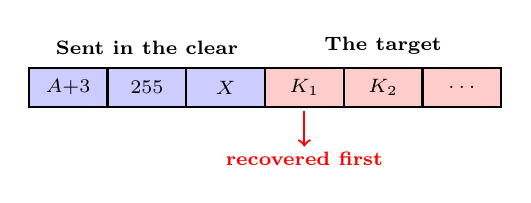
\begin{tikzpicture}[scale=0.5]
					\draw[thick, fill=blue!20] (0,2) rectangle (2,3);
					\node at (1,2.5) {\scriptsize $A{+}3$};
					\draw[thick, fill=blue!20] (2,2) rectangle (4,3);
					\node at (3,2.5) {\scriptsize $255$};
					\draw[thick, fill=blue!20] (4,2) rectangle (6,3);
					\node at (5,2.5) {\scriptsize $X$};
					\draw[thick, fill=red!20] (6,2) rectangle (8,3);
					\node at (7,2.5) {\scriptsize $K_1$};
					\draw[thick, fill=red!20] (8,2) rectangle (10,3);
					\node at (9,2.5) {\scriptsize $K_2$};
					\draw[thick, fill=red!20] (10,2) rectangle (12,3);
					\node at (11,2.5) {\scriptsize $\ldots$};
					\node[above] at (3,3.1) {\textbf{\scriptsize Sent in the clear}};
					\node[above] at (9,3.1) {\textbf{\scriptsize The target}};
					\draw[->, thick, red] (7,1.9) -- (7,1.0);
					\node[below, red] at (7,1.1) {\textbf{\scriptsize recovered first}};
				\end{tikzpicture}
			\end{center}
			\onslide<+->{
				\alertbox{Note what is \emph{not} needed}{
					No brute force. No cryptographic assumption. No interaction with the network. Just listening, and arithmetic.
				}
			}
		\end{column}
	\end{columns}
\end{frame}

\begin{frame}{Why $(A+3, 255, X)$? Let us trace it}
	\begin{columns}[c]
		\begin{column}{0.52\textwidth}
			Take $A = 0$, so $IV = (3, 255, X)$. Every step below depends only on the \emph{public} IV, so the attacker can replay it.
			\begin{center}
				\footnotesize
				\renewcommand{\arraystretch}{0.9}
				\begin{tabular}{|c|l|l|}
					\hline
					$i$ & $j$ becomes         & effect                                          \\
					\hline
					0   & $0 + 0 + 3 = 3$     & $S[0]=3,\ S[3]=0$                               \\
					1   & $3 + 1 + 255 = 3$   & $S[1]=0,\ S[3]=1$                               \\
					2   & $3 + 2 + X = X{+}5$ & touches $S[2], S[X{+}5]$                        \\
					3   & $X{+}6+K_1 $        & \textcolor{red}{$S[3] \coloneq S[X{+}6{+}K_1]$} \\
					\hline
				\end{tabular}
			\end{center}
			First PRGA step: $i = 1$, $j = S[1] = 0$, so swap $S[1]$ with $S[0]$ and emit $Z_1 = S[S[1] {+} S[0]] = S[3]$.
		\end{column}
		\begin{column}{0.48\textwidth}
			\begin{itemize}[<+->]
				\item The first keystream byte \textbf{is} whatever step $i=3$ deposited at $S[3]$, and it came from index $X + 6 + K_1$. The attacker replayed the permutation, so they invert it: $K_1 = S_3^{-1}[Z_1] - X - 6$.
				\item This holds only if the remaining $252$ KSA steps never touch indices $0, 1, 3$: probability $\approx e^{-3} \approx \textbf{5\%}$.
				\item The other $95\%$ is evenly spread noise. \textbf{So take a vote:} the true $K_1$ polls $\approx 5\%$, each wrong value $\approx 0.4\%$.
			\end{itemize}
		\end{column}
	\end{columns}
\end{frame}

\begin{frame}{From paper to practice, in months}
	\begin{itemize}[<+->]
		\item \textbf{August 2001:} the FMS paper appears at Selected Areas in Cryptography.
		\item \textbf{August 2001:} Stubblefield, Ioannidis and Rubin implement it and pull a real key off a real access point, in a paper titled \textit{Using the Fluhrer, Mantin, and Shamir Attack to Break WEP}.
		\item \textbf{Weeks later:} \textbf{AirSnort} and \textbf{WEPCrack} ship as free public tools. Point, click, wait for a few million packets, get the key.
		\item \textbf{2004--2006:} \textbf{aircrack-ng} adds \textbf{packet injection} --- replay an ARP request and the access point generates traffic on demand. The attacker stops waiting for a busy network and manufactures the traffic instead.
	\end{itemize}
	\onslide<+->{\centering\textbf{From ``interesting theoretical result'' to script-kiddie tool: about three months.}}
\end{frame}

\begin{frame}{Attacks only get better}
	\begin{columns}[c]
		\begin{column}{0.54\textwidth}
			\begin{itemize}[<+->]
				\item \textbf{Klein:} a stronger key--keystream correlation that does \emph{not} need the special FMS IV shape. Suddenly \emph{every} packet is useful, not one in $2^{16}$.
				\item \textbf{PTW --- Tews, Weinmann and Pyshkin (2007):} combine Klein's correlation with Bayesian ranking of candidate key bytes, attacking all bytes at once instead of left to right.
				      \begin{itemize}
					      \item \textbf{40{,}000} packets for $50\%$ success, \textbf{85{,}000} for $95\%$.
					      \item Paper title: \textit{Breaking 104 bit WEP in less than 60 seconds}.
				      \end{itemize}
			\end{itemize}
		\end{column}
		\begin{column}{0.46\textwidth}
			\onslide<+->{
				\definitionbox{The trend line is the lesson}{
					\textbf{2001:} millions of packets, hours of collection.
					\\[0.2em]
					\textbf{2005:} hundreds of thousands.
					\\[0.2em]
					\textbf{2007:} tens of thousands, under a minute.
					\\[0.5em]
					Nobody found a \emph{new} weakness in RC4 between 2001 and 2007. They just got better at using the one they had.
				}
			}
			\onslide<+->{\centering\textit{``Attacks always get better; they never get worse.''}}
		\end{column}
	\end{columns}
\end{frame}

\begin{frame}{What WEP got wrong}
	\begin{itemize}[<+->]
		\item \textbf{It fed attacker-visible data straight into the key.} Concatenating a public IV with a secret key is not key derivation. WPA2 and everything since run a \textbf{KDF}, so per-packet keys are unrelated even when their inputs are not.
		\item \textbf{It reused one key across every device and every packet.} No forward secrecy, no isolation: one compromise is total compromise.
		\item \textbf{It chose a 24-bit IV.} Even with perfect key derivation, that space exhausts in hours.
		\item \textbf{It had no real integrity protection.} WEP's CRC-32 checksum is linear, so an attacker can flip ciphertext bits and patch the checksum to match.
	\end{itemize}
	\onslide<+->{\centering\textbf{None of this is RC4's fault.} WEP would still be broken had it used AES this way.}
\end{frame}

\section{RC4 in TLS}

\begin{frame}{The BEAST irony (2011)}
	\begin{itemize}[<+->]
		\item By 2011, TLS deployments had two realistic choices: \textbf{AES in CBC mode}, or \textbf{RC4}.
		\item Then \textbf{BEAST} broke CBC in TLS 1.0 --- a chosen-plaintext attack on predictable CBC initialisation vectors, able to decrypt cookies out of a live browser session.
		\item The industry's advice was immediate and near-unanimous: \textbf{switch to RC4}. It is a stream cipher, so there are no CBC IVs, no padding, and no padding oracles.
		\item It worked, and RC4 usage \emph{rose sharply} --- to roughly half of all TLS traffic.
	\end{itemize}
	\onslide<+->{
		\alertbox{The trap}{
			RC4's biases were public, peer-reviewed and a decade old, but were dismissed as ``theoretical'' because the sample counts looked impossibly large. Nobody checked whether the modern web could supply them. Fleeing one attack drove the industry into another.
		}
	}
\end{frame}

\begin{frame}{AlFardan et al. (2013): the biases are real, and reachable}
	\begin{columns}[c]
		\begin{column}{0.52\textwidth}
			\begin{itemize}[<+->]
				\item Rather than reason analytically, five researchers \emph{measured} RC4's keystream over a vast number of random keys.\footnote{\url{https://appliedcryptography.page/paper/\#rc4-tls}} The biases are not confined to byte 2: \textbf{every one} of the first 256 positions is non-uniform.
				\item $2^{26}$ sessions recovered the first $\approx 40$ bytes of application data at over $50\%$ per byte; $2^{32}$ got essentially all $256$.
				\item None of this needs a weak key: these are properties of the algorithm.
			\end{itemize}
		\end{column}
		\begin{column}{0.48\textwidth}
			\onslide<+->{
				\definitionbox{Two families of bias}{
					\textbf{Single-byte:} at a fixed position $r \leq 256$, some values of $Z_r$ beat $1/256$. Strong, but only near the start.
					\vspace{0.4em}
					\\
					\textbf{Double-byte (Fluhrer--McGrew):} certain \emph{pairs} $(Z_r, Z_{r+1})$ beat $1/256^2$, by only $\approx 1/256$ relative --- but \textbf{everywhere} in the keystream, not just the start.
				}
			}
		\end{column}
	\end{columns}
\end{frame}

\begin{frame}{The broadcast attack}
	\begin{columns}[c]
		\begin{column}{0.56\textwidth}
			\begin{itemize}[<+->]
				\item \textbf{The setting:} one plaintext, encrypted under many \emph{independent} keys. TLS derives a fresh key per connection, so this is the normal case, not a misuse.
				\item \textbf{The web supplies it for free:} a session cookie sits at a fixed offset in every request your browser makes.
				\item \textbf{The attack:} collect $C^{(1)}, \ldots, C^{(n)}$ and, for each position $r$, tally the most frequent byte. Since $C_r = M_r \oplus Z_r$, the bias in $Z_r$ shows through as a bias in $C_r$, pointing straight at $M_r$. \textbf{No key is ever recovered.}
			\end{itemize}
		\end{column}
		\begin{column}{0.44\textwidth}
			\onslide<+->{
				\definitionbox{Why counting works}{
					Telling a coin with bias $\varepsilon$ from a fair one takes about $1/\varepsilon^2$ flips.
					\vspace{0.4em}
					\\
					Halve the bias and you \emph{quadruple} the samples --- but you never make the attack impossible, only expensive.
				}
			}
			\onslide<+->{\centering And the attacker controls $n$: inject JavaScript into any page the victim loads and it will issue requests all day. ``Needs $2^{30}$ ciphertexts'' is a claim about \emph{time}, not feasibility.}
		\end{column}
	\end{columns}
\end{frame}

\begin{frame}{Mantin's ABSAB bias (2005)}
	\begin{columns}[c]
		\begin{column}{0.54\textwidth}
			\begin{itemize}[<+->]
				\item A different shape of weakness: not ``this byte is biased'' but \textbf{``this byte repeats too often.''}\footnote{\url{https://appliedcryptography.page/paper/\#rc4-absab}}
				\item A digraph $AB$ tends to reappear $G$ positions later, forming $AB\!\ldots\!AB$. In a random keystream that has probability $1/N^2$ with $N = 256$; in RC4 it is $\frac{1}{N^2}\left(1 + \frac{e^{(-4-8G)/N}}{N}\right)$.
				\item That is a relative bias of about $1/N$ at zero gap, decaying as the gap grows.
			\end{itemize}
		\end{column}
		\begin{column}{0.46\textwidth}
			\onslide<+->{
				\definitionbox{Why this one matters most}{
					Single-byte biases live in the first 256 bytes, so TLS could have escaped them by discarding the keystream's start. ABSAB is a \textbf{long-term} bias, present at position 10 and at position 10 million: there is no prefix you can throw away.
					\vspace{0.4em}
					\\
					It also relates a byte to \emph{another byte of the same plaintext} --- exactly what you want against something structured, like a password.
				}
			}
		\end{column}
	\end{columns}
\end{frame}

\begin{frame}{2015: three attacks finish the job}
	\begin{itemize}[<+->]
		\item \textbf{``Bar Mitzvah'' (Mantin, Black Hat Asia).} Revisits the \textbf{invariance weakness} that Fluhrer, Mantin and Shamir had described back in 2001: for a class of weak keys, structure in the key survives the KSA and leaks plaintext. The name is a joke about a weakness finally coming of age at thirteen.
		\item \textbf{Garman, Paterson and van der Merwe (USENIX Security),} \textit{Attacks Only Get Better}.\footnote{\url{https://appliedcryptography.page/paper/\#rc4-attacks}}
		      \begin{itemize}
			      \item Target \textbf{passwords} rather than cookies: HTTP Basic Authentication and IMAP resend the password on \emph{every} request.
			      \item Combine the ABSAB bias with how humans actually choose passwords, plus a dictionary.
		      \end{itemize}
		\item \textbf{Vanhoef and Piessens, ``RC4 NOMORE'' (USENIX Security).} The same machinery, actually executed: a real browser cookie decrypted in \textbf{52 hours}, and \textbf{WPA-TKIP} --- WEP's own RC4-based replacement --- broken in about \textbf{one}.\footnote{\url{https://appliedcryptography.page/paper/\#rc4-biases}}
	\end{itemize}
	\onslide<+->{\centering\textbf{After this, no serious argument for keeping RC4 remained.}}
\end{frame}

\begin{frame}{Why passwords were the softer target}
	\begin{columns}[c]
		\begin{column}{0.56\textwidth}
			\begin{itemize}[<+->]
				\item A cookie is high-entropy and random. Statistics has to recover \textbf{every byte} correctly, unaided.
				\item A password is not random at all:
				      \begin{itemize}
					      \item Drawn from a small, heavily skewed alphabet, and base64-encoded in Basic Auth --- which shrinks it further and imposes a rigid known format.
					      \item Very likely to appear in some leaked password list.
				      \end{itemize}
				\item So the attacker never has to \emph{recover} the password --- only narrow the candidates until a dictionary finishes.
			\end{itemize}
		\end{column}
		\begin{column}{0.44\textwidth}
			\onslide<+->{
				\alertbox{The general principle}{
					Statistical attacks and structural knowledge \textbf{multiply}. Every byte of context you have is a byte the statistics no longer has to earn.
					\vspace{0.4em}
					\\
					So ``the attack needs $2^{n}$ samples'' is never the end of the analysis. It is the cost \emph{before} anyone gets clever.
				}
			}
		\end{column}
	\end{columns}
\end{frame}

\begin{frame}{The long goodbye}
	\begin{itemize}[<+->]
		\item \textbf{2013:} AlFardan et al. lands. The IETF opens the deprecation discussion; Microsoft, Google and Mozilla start advising against RC4.
		\item \textbf{2014:} \textbf{POODLE} kills SSL 3.0. Not an RC4 attack --- but SSL 3.0's only other option was CBC, so between POODLE and the biases, \textbf{SSL 3.0 had no safe cipher left at all}.\footnote{\url{https://appliedcryptography.page/paper/\#google-poodle}}
		\item \textbf{February 2015: RFC 7465}, \textit{Prohibiting RC4 Cipher Suites}: ``TLS clients MUST NOT include RC4 cipher suites'' and ``TLS servers MUST NOT select an RC4 cipher suite.''
		\item \textbf{September 2015:} Google, Mozilla and Microsoft announce removal \emph{on the same day}, so that no single browser would take the blame for breaking sites. Chrome 48 and Firefox 44 ship it in January 2016; Microsoft follows that August.
	\end{itemize}
	\onslide<+->{\centering\textbf{Fourteen years from first practical break to removal.} Deprecating a cipher is a social problem at least as much as a technical one.}
\end{frame}

\section{What RC4 Teaches Us}

\begin{frame}{Six lessons}
	\begin{itemize}[<+->]
		\item \textbf{1. A primitive's interface is part of its security.} RC4's missing nonce was not a bug in any line of its code, and it caused both catastrophes.
		\item \textbf{2. Small biases are not small.} A $2^{-8}$ relative bias sounds negligible until the attacker has $2^{30}$ samples --- and the modern web hands out samples for free.
		\item \textbf{3. ``Theoretical'' means ``practical, later.''} FMS to AirSnort took three months. Mantin--Shamir to a TLS break took twelve years, but it arrived.
		\item \textbf{4. Attacks compose.} Bias plus password structure. Downgrade plus weak cipher. Results are components, and components multiply.
		\item \textbf{5. Fleeing an attack is not a strategy.} BEAST pushed the industry out of a broken mode and into a broken cipher. Have somewhere \emph{good} to run to.
		\item \textbf{6. Plan the exit before you need it.} \textbf{Cryptographic agility} --- negotiating algorithms, and being able to remove them --- has to be designed in from day one.
	\end{itemize}
\end{frame}

\begin{frame}{What replaced RC4, and why it fails differently}
	\begin{columns}[c]
		\begin{column}{0.54\textwidth}
			\begin{itemize}[<+->]
				\item \textbf{It takes a nonce.} Protocols no longer improvise per-message keys, so WEP's mistake is not even expressible.
				\item \textbf{It has no evolving secret state.} Each block is an independent function of $(K, N, \text{ctr})$: no long-lived permutation to leak, no key schedule whose residue shows up in the output.
				\item \textbf{It comes bolted to a MAC.} \textbf{ChaCha20-Poly1305} is AEAD, so WEP's forgeable CRC-32 could not happen.
			\end{itemize}
		\end{column}
		\begin{column}{0.46\textwidth}
			\onslide<+->{
				\definitionbox{The structural difference}{
					RC4 says: \emph{stir a secret state, and dribble out bytes of it.}
					\vspace{0.4em}
					\\
					ChaCha20 says: \emph{apply a strong public function to a counter, keyed by the secret.}
					\vspace{0.4em}
					\\
					The second is a PRF evaluated at distinct points --- a design we know how to reason about, and the same shape as AES-CTR.
				}
			}
			\onslide<+->{\centering TLS 1.3 ended the argument by deleting the choice: only AEAD ciphers remain.}
		\end{column}
	\end{columns}
\end{frame}

\begin{frame}{RC4 is dead. RC4 is still running.}
	\begin{itemize}[<+->]
		\item \textbf{Kerberos.} The \texttt{RC4-HMAC} encryption type shipped in Windows domains for two decades. Microsoft has spent years disabling it, and ``Kerberoasting'' against RC4 tickets remains a routine penetration-test finding.
		\item \textbf{Documents and firmware.} Older Office and PDF encryption used RC4, and devices shipped in 2008 still run today. Neither will ever be updated.
		\item \textbf{Recorded traffic.} Anyone who archived RC4-protected sessions in 2013 can attack them at leisure today. Deprecation does not protect the past.
	\end{itemize}
	\onslide<+->{
		\alertbox{The real lesson about deprecation}{
			An algorithm dies when its last deployment stops, not when the RFC is published --- and those can be decades apart. Judge the cost of adopting an algorithm by how hard it will be to remove.
		}
	}
\end{frame}

\begin{frame}{RC4: a complete timeline}
	\begin{columns}[c]
		\begin{column}{0.5\textwidth}
			\begin{itemize}
				\item \textbf{1987:} Rivest designs RC4.
				\item \textbf{1994:} Leaked to Cypherpunks.
				\item \textbf{1995:} Roos finds weak keys.
				\item \textbf{1996--97:} Glimpse theorem; Goli\'{c}'s distinguisher.
				\item \textbf{1997:} WEP standardises on RC4.
				\item \textbf{2001:} Mantin--Shamir second-byte bias.
				\item \textbf{2001:} FMS attack, then AirSnort. WEP is over.
				\item \textbf{2003--04:} WPA, then WPA2 with AES.
			\end{itemize}
		\end{column}
		\begin{column}{0.5\textwidth}
			\begin{itemize}
				\item \textbf{2005:} ABSAB bias; Klein's attack.
				\item \textbf{2007:} PTW breaks WEP in under a minute.
				\item \textbf{2011:} BEAST \emph{increases} RC4 usage.
				\item \textbf{2013:} AlFardan et al. break RC4 in TLS.
				\item \textbf{2014:} POODLE leaves SSL 3.0 with nothing safe.
				\item \textbf{2015:} Bar Mitzvah, Garman et al., RC4 NOMORE.
				\item \textbf{2015:} RFC 7465 prohibits RC4 in TLS.
				\item \textbf{2016:} Removed from major browsers.
			\end{itemize}
		\end{column}
	\end{columns}
	\centering\textbf{Twenty years of published warnings between the first crack and the ban.}
	\vspace{-0.5em}
\end{frame}

\begin{frame}{Discussion time}
	\begin{columns}[c]
		\begin{column}{0.68\textwidth}
			\begin{enumerate}
				\item \textbf{When is a cipher ``broken''?}
				      \begin{itemize}
					      \item In 2001 RC4 failed our formal definition; in 2013 it failed in practice. Which year should have triggered removal?
				      \end{itemize}
				\item \textbf{Was the flight to RC4 after BEAST a mistake?}
				      \begin{itemize}
					      \item It was the consensus advice of competent people, given what they knew. What would you have recommended?
				      \end{itemize}
				\item \textbf{Who owns the fourteen-year gap?}
				      \begin{itemize}
					      \item Academics who called their own attacks impractical? Vendors afraid of breaking sites? Standards bodies?
				      \end{itemize}
				\item \textbf{What are we doing right now that will look like this in 2040?}
			\end{enumerate}
		\end{column}
		\begin{column}{0.32\textwidth}
			\imagewithcaption{spamton-sez.png}{}
		\end{column}
	\end{columns}
\end{frame}

\begin{frame}[plain]
	\titlepage
\end{frame}
\end{document}
